
\clearpage

\appendix

\section{Appendix}

\subsection{FPGA Resource Utilization}

The following table shows the FPGA resources used by \snic{} shell.
Most of the resources are left for running \nt{}s.

\begin{center}
\scriptsize
\begin{tabular}{ p{0.6in} | p{0.2in} |p{0.27in} }
 & \textbf{Logic} & \textbf{Memory} \\
\textbf{Module} & \textbf{(LUT)} & \textbf{(BRAM)} \\
\hline
\hline
%Firewall     & 2.8\% & 0.5\% \\
%AES-256       & 0.4\% & 0 \\
%Transport    & 1.3\% & 0.42\% \\
%\hline
%\hline
\snic{} Core & 4.36\%   & 4.74\% \\
Packet Store & 0.91\%   & 9.17\% \\
PHY+MAC      & 0.72\%   & 0.35\% \\
DDR4Controller         & 1.57\%   & 0.29\% \\
MicroBlaze   & 0.25\%   & 1.81\% \\
Misc         & 1.52\%   & 0.75\% \\
%\textbf{Total (w/o \nt{})}        & \textbf{9.33\%}   & \textbf{17.11\%} \\
\hline
\textbf{Total}        & \textbf{9.33\%}   & \textbf{17.11\%} \\
\end{tabular}
\end{center}



\subsection{Cost Calculation}
We explain the different deployment models and the cost calculation formulas behind our CapEx comparisons.
We limit our scope to rack-scale as the higher-level network hierarchies
are orthogonal to the resource pool deployment models.
We calculate that, to deploy a certain number of endpoints, what's the
network cost (i.e., the network interface card, cable, and switch port costs).

We compare the following models:
1) Non-disaggregation model, or the traditional model, termed \texttt{traditional}.
2) Disaggregation model, in which we insert the network pool between endpoints and the ToR switch (Figure~\ref{fig-topology} (a)), termed \texttt{ring}.
3) Disaggregattion model, in which we connect the pool of network devices directly to the ToR switch (Figure~\ref{fig-topology} (b)), termed \texttt{direct}.
For both disaggregation models, we further compare two type of devices: sNIC which has auto-scaling capability and multi-host NIC which can only provision for max resource usage. With runtime dynamic scaling and load balancing features, sNICs can provision for less than the max required resource , the specific ratio is calculated by comparing a particular workload's the sum-of-peak versus the peak-of-sum.

In all, we have the following models under comparison:
\texttt{traditionl, sNIC-direct, sNIC-ring, mhnic-direct, mhnic-ring}.

We now detail the cost calculations.
In the traditional non-disaggregation model,
each endpoint has a full-fledged NIC and a normal high-speed cable for connection to the ToR switch.
In both disaggregation models, since most network tasks are offloaded to the network resource pool, each endpoint can uses a down-scaled NIC.
Furthermore, the last hop link layer between endpoints and the network resource pool is reliable, we can leverage down-scaled, cheaper and less reliable physical cable~\cite{RAIL-NSDI}.

We use the following parameters in our calculation:
\begin{itemize}
\item Deploy \texttt{N} devices.
\item Each switch port has a cost of \texttt{costSwitchPort}
\item A full-fledged NIC's cost is \texttt{costNIC}. A down-scaled NIC cost is \texttt{costDSNIC}.
\item A normal high-speed cable cost is \texttt{costCable}.
A down-scaled less reliable physical cable cost is \texttt{costDSCable}.
\item A consolidation ratio \texttt{consolidRatio} determines how many endpoints are sharing one network resource pool device. We can calculate the number of network pool devices by \texttt{M = N / consolidRatio}.
\item For a network device, only a certain portion is dedicated to running network task, other parts are used as shell. We define the cost ratio used by network task to be \texttt{NTCostRatio}.
\item The peak-of-sum versus the sum-of-peak yields the auto-scaling potentials. A multi-host NIC (mhnic) provisions for the sum-of-peak while an sNIC provisions for the peak-of-sum. We call this ratio \texttt{capExConsolidRatio}.
\item The multi-host NIC's cost can be calculated as \texttt{costMHNIC = costNIC * N}.
\item The sNIC's cost can be calculated as \texttt{costsNIC = costMHNIC * capExRatio}, in which \texttt{capExRatio = (1 - NTCostRatio) + NTCostRatio * capExConsolidRatio}.
\end{itemize}

We now define each model's cost.

The traditional deployment model's cost is straightforward, it includes NIC, cable and switch ports:
\begin{gather}
N * (costNIC + costCable + costSwitchPort)
\end{gather}

The disaggregation models' cost has more moving parts than the traditional. It includes the down-scaled NICs and cables, network pool devices, the cables to the ToR switch, and switch ports.

The first disaggregation model (Figure~\ref{fig-topology} (a)) can be calculated as follows (for both \texttt{sNIC-ring, mhnic-ring}). 
\begin{align}
N * (costDSNIC + costDSCable) + \\
M * (costsNIC + costCable + costSwitchPort)
\end{align}

The second disaggregation model (Figure~\ref{fig-topology} (b)) can be calculated as follows (for both \texttt{sNIC-direct, mhnic-direct}).
\begin{align}
N * (costDSNIC + costCable + costSwitchPort) + \\
M * (costsNIC + costCable + costSwitchPort)
\end{align}

This tables shows the real-world numbers we use.

\begin{center}
\scriptsize
\begin{tabular}{|l|l|l|} 
 \hline
 Parameters & Value & Note \\
 \hline\hline
 costSwitchPort & \$250 & FS 100Gbps switch~\cite{fs-64port-switch} \\
 costNIC & \$500 & Mellanox Connect-X5 \\
 costCable & \$100 & FS DAC 100Gbps cable \\
 costDSNIC & costNIC * 0.2 & Numbers from our prototpe \\
 costDSCable & costCable * 0.6 & ~\cite{RAIL-NSDI} \\
 consolidRatio & 4 & Current model\\
 NTCostRatio & 0.9 & Numbers from our prototype \\
 capExConslidRatio & 0.23 & Facebook Hadoop trace~\cite{facebook-sigcomm15} \\
 \hline
\end{tabular}
\end{center}

%\subsection{Extended Evaluation Results}

{
\begin{figure*}[th]
\begin{minipage}{\figWidthSix}
\begin{center}
\centerline{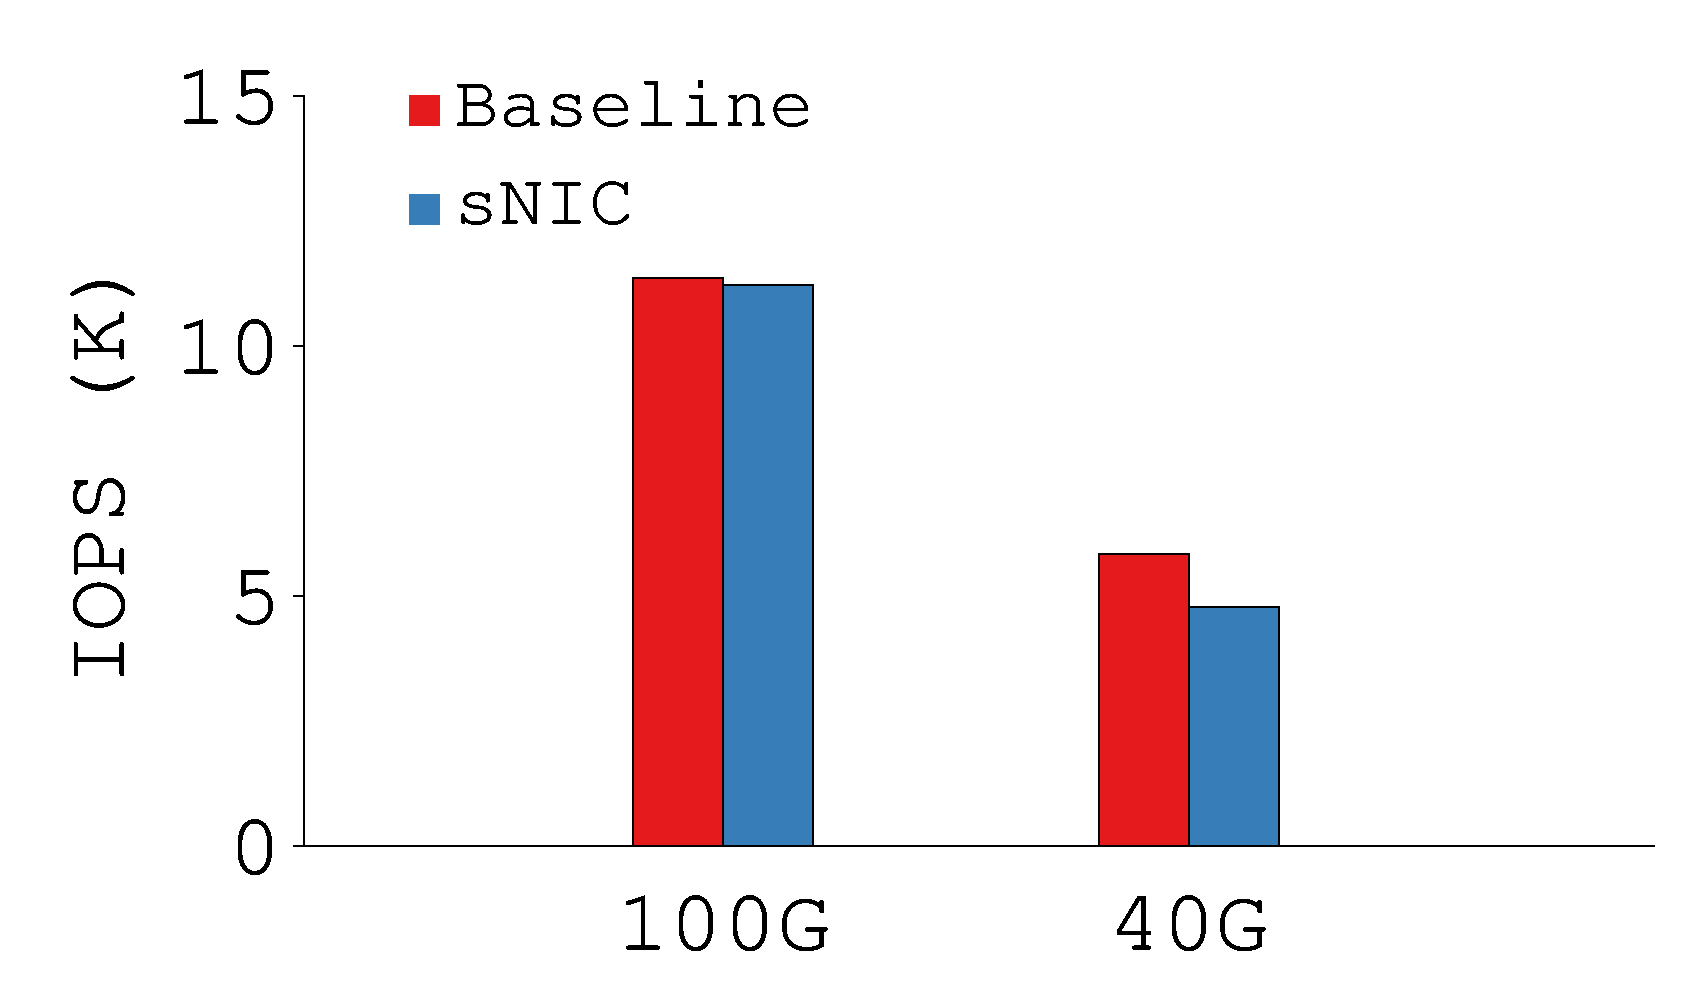
\includegraphics[width=\columnwidth]{Figures/g_plot_conslid_perf.pdf}}
\vspace{-0.1in}
\mycaption{fig-kv-consolid}{Consolidation Performance w/ FB Key-Value.}
{
}
\end{center}
\end{minipage}
\begin{minipage}{\figWidthSix}
\begin{center}
\centerline{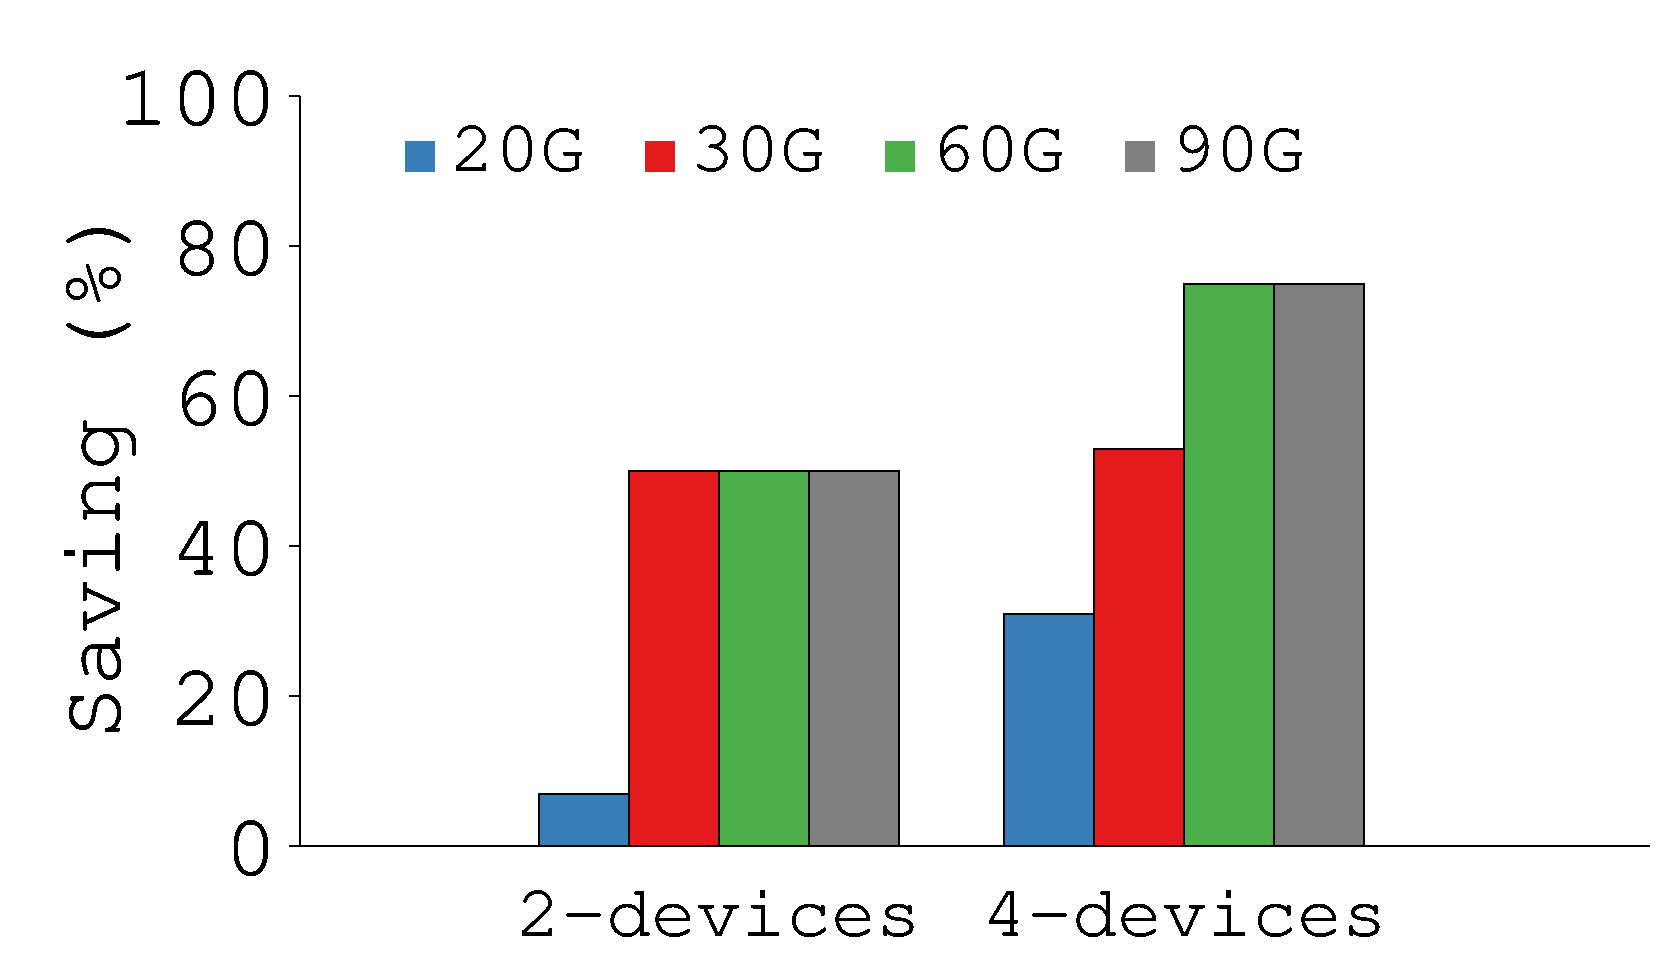
\includegraphics[width=\columnwidth]{Figures/g_plot_conslid_cost.pdf}}
\vspace{-0.1in}
\mycaption{fig-kv-cost}{Consolidation Resource Usage w/ FB KV.}
{
}
\end{center}
\end{minipage}
\vspace{-0.1in}
\end{figure*}
}
\subsection{End-to-End Application Performance and Cost with Consolidation}

To evaluate the benefit and tradeoff of consolidation, we deploy a testbed with four sender and four receiving servers with four setups:
each endhost connects to a ToR switch with 100\Gbps\ or 40\Gbps\ link (baseline, no consolidation), and four endhosts connect to an \snic, each with 100\Gbps\ or 40\Gbps\ link, and the \snic\ connects to the ToR switch with a 100\Gbps\ or 40\Gbps\ link (\snic\ consolidation).
%, and 3) four endhosts connect to an emulated multi-host NIC, each with a 25\Gbps\ link (\S\ref{sec:related}), and the multi-host NIC connects to the ToR switch with a 100\Gbps\ link. %(multi-host NIC, statically partitioned link bandwidth).
For both settings, we execute two \nt{}s, firewall and NAT, in FPGA. 
For the baseline, each endhost has its own set of \nt{}s, while %the multi-host NIC uses one set of \nt{}s in total and 
\snic\ autoscales \nt{}s as described in \S\ref{sec:policy}.
On each server, we generate traffic to follow inter-arrival and size distribution reported in the Facebook 2012 key-value store trace~\cite{Atikoglu12-SIGMETRICS}.
%the Hadoop load distribution reported in the 2015 Facebook workloads~\cite{facebook-sigcomm15}.
%Since there is no reported inter-arrival time for these workloads, we use the inter-arrival time reported by the 2012 Facebook workloads~\cite{Atikoglu12-SIGMETRICS}.
%We measure the application throughput (IOPS) every 10\ms\ time unit to evaluate the throughput changes over time.

Figure~\ref{fig-kv-consolid} reports the throughput comparison of \snic\ and the baseline.
%average IOPS and 95-percentile IOPS across all time units for the three settings. 
\snic\ only adds 1.3\% performance overhead to the baseline under 100\Gbps\ network and 18\% overhead under 40\Gbps\ network. 
We further analyze the workload and found its median and 95-percentile loads to be 24\Gbps\ and 32\Gbps.
With four senders/receivers, the aggregated load is mostly under 100\Gbps\ but often exceeds 40\Gbps.
Note that a multi-host NIC would not be able to achieve \snic's performance, as it subdivides the 100\Gbps\ or 40\Gbps\ into four 25\Gbps\ or 10\Gbps\ sub-links, which would result in each endhost exceeding its sub-link capacity.


We then calculate the amount of FPGA used for running the \nt{}s multiplied by the duration they are used for, to capture the run-time resource consumption with \snic's autoscaling mechanism. The baseline has one set of \nt{}s per endhost for the whole duration.
Figure~\ref{fig-kv-cost} shows this comparison when consolidating two and four endhosts to an \snic\ and using \nt{}s of different performance metrics.
For a slower \nt{} (\eg, one that can only sustain 20\Gbps\ max load), the \snic\ auto-scales more instances of it, resulting in less cost saving.
Our implementation of firewall \nt{} reaches 100\Gbps, while the AES \nt\ is 30\Gbps, resulting in a 64\% cost saving when deploying both of them.



%On the other hand, multi-host NIC incurs higher performance overhead, especially for the tail.
%Whenever any endhost exceeds 25\Gbps\ load, multi-host NIC will have a bottleneck link.
%On the other hand, \snic\ can sustain the peak of aggregated traffic, which is mostly under 100\Gbps, demonstrating the benefit of run-time, dynamic consolidation.

\if 0
\subsubsection{Distributed \snic{}}
To run an \nt\ at a remote \snic,
an \snic{}'s SoftCore first sends a control message to the remote \snic{} to launch the \nt{} and then installs forwarding rules to its parser. This process takes 2.3\mus\ in our testbed.
Afterwards, packets are forwarded to the remote \snic. We observe an addition of 1.3\mus\ latency when packets go through the remote \snic.
\fi